\documentclass[a4paper, 10pt]{article}
\usepackage{../../CEDT-Homework-style}

\usepackage{amsmath}
\allowdisplaybreaks

\setlength{\headheight}{14.49998pt}

\begin{document}
\subject[2110203 - Computer Engineering Mathematics II]
\hwtitle{Signal 3}{}{Week 3}{6733172621 Patthadon Phengpinij}{ChatGPT (for\,\LaTeX\,styling and grammar checking)}


% ================================================================================ %
\section{Fourier Series}
% ================================================================================ %



% ================================================================================ %
%                                    Problem 02                                    %
% ================================================================================ %
\begin{problem}[2]
Find the Fourier Series (FS) of the periodic function \( x(t) \) which are provided as follows.
\end{problem}


% === Problem 2.2. === %
\begin{tosubmit}
\begin{subproblems}[start=2]
    \item \( x(t) = \pi - t;\; -\pi \leq t \leq \pi \)
\end{subproblems}

\par\noindent\submitsolution
To find the Fourier series of the function \( x(t) = \pi - t \) for \( -\pi \leq t \leq \pi \), we first need to compute the Fourier coefficients.
The Fourier coefficients \( a_k \) are given by:
\[ a_k = \frac{1}{T} \int_{\langle T \rangle} x(t) e^{-j k \omega_0 t} \,dt \]

where \( T = 2\pi \) (the period of the function).

Calculating \( \omega_0 \):
\[ \omega_0 = \frac{2 \pi}{T} = \frac{2\pi}{2\pi} = 1 \]

Calculating \( a_0 \):
\begin{align*}
    a_0 &= \frac{1}{T} \int_{\langle T \rangle} x(t) e^{-j (0) \omega_0 t} \,dt \\
    &= \frac{1}{2\pi} \int_{-\pi}^{\pi} (\pi - t) \,dt \\
    &= \frac{1}{2\pi} \sqbracket{ \pi t - \frac{t^2}{2} }_{-\pi}^{\pi} \\
    &= \frac{1}{2\pi} \paren{ \pi^2 - \frac{\pi^2}{2} - (-\pi^2 - \frac{\pi^2}{2}) } \\
    a_0 &= \pi
\end{align*}

Calculating \( a_k \) for \( k \neq 0 \):
\begin{align*}
    a_0 &= \frac{1}{T} \int_{\langle T \rangle} x(t) e^{-j k \omega_0 t} \,dt \\
    &= \frac{1}{2\pi} \int_{-\pi}^{\pi} (\pi - t) e^{-j k t} \,dt \\
    a_k &= \frac{1}{2\pi} \sqbracket{ \pi \int_{-\pi}^{\pi} e^{-j k t} \,dt - \int_{-\pi}^{\pi} t e^{-j k t} \,dt }
\end{align*}

To solve the integral, we can use integration by parts multiple times.
Using tabular integration by parts, we find:

\renewcommand{\arraystretch}{1.7}
\[
\begin{array}{c:c|c}
    \text{Sign} & \text{Derivative} & \text{Integral} \\
    \hline
    \hline
    + & t & e^{-j \pi k t} \\
    - & 1 & \frac{1}{-j \pi k} e^{-j \pi k t} \\
    + & 0 & \frac{1}{(-j \pi k)^2} e^{-j \pi k t} \\
    \hline
\end{array}
\]

Thus, we have:
\[ \int t e^{-j k t} \,dt = \frac{t}{-j k} e^{-j k t} - \frac{1}{(-j k)^2} e^{-j k t} \]

\newpage

Evaluating this from \( -\pi \) to \( \pi \) to find \( a_k \):
\begin{align*}
    a_k &= \frac{1}{2\pi} \sqbracket{ \pi \sqbracket{ \frac{e^{-j k t}}{-j k} }_{-\pi}^{\pi} - \sqbracket{ \frac{t}{-j k} e^{-j k t} - \frac{1}{(-j k)^2} e^{-j k t} }_{-\pi}^{\pi} } \\
    &= \frac{1}{2} \sqbracket{ \frac{e^{-j k t}}{-j k} }_{-\pi}^{\pi} - \frac{1}{2\pi} \sqbracket{ \frac{t}{-j k} e^{-j k t} - \frac{1}{(-j k)^2} e^{-j k t} }_{-\pi}^{\pi} \\
    &= \frac{1}{2} \sqbracket{ \frac{ \paren{ e^{-j \pi k} - e^{j \pi k} } }{-j k} } - \frac{1}{2\pi} \sqbracket{ \frac{ \paren{ \pi e^{-j \pi k} + \pi e^{j \pi k} } }{-j k} - \frac{ \paren{ e^{-j \pi k} - e^{j \pi k} } }{(-j k)^2} } \\
    &= \frac{1}{\cancel{2}} \sqbracket{ \frac{ \paren{ -\cancel{2} \bcancel{j} \sin{\pi k} } }{- \bcancel{j} k} } - \frac{1}{\cancel{2}\pi} \sqbracket{ \frac{ \paren{ \cancel{2}\pi \cos{\pi k} } }{-j k} - \frac{ \paren{ -\cancel{2}j\sin{\pi k} } }{(-j k)^2} } \\
    a_k &= \frac{ \sin{\pi k} }{n} + \frac{ \cos{\pi k} }{jn} - \frac{ \sin{\pi k} }{j\pi k^2}
\end{align*}

\newpage

We can simplify \( a_k \):
\[
a_k = 0 + \frac{ (-1)^k }{jk} - 0 = \frac{ (-1)^k }{jk} \text{ for } k \neq 0
\]

Thus, the Fourier series expansion of \( x(t) \) is:
\[ \boxed{ x(t) = \pi + \sum_{k \neq 0} \frac{(-1)^k}{jk} e^{j k t}} \]

By using Fourier series and Python approximation with \( N = 10 \) harmonics, we can approximate the signal as follows:
\begin{center}
    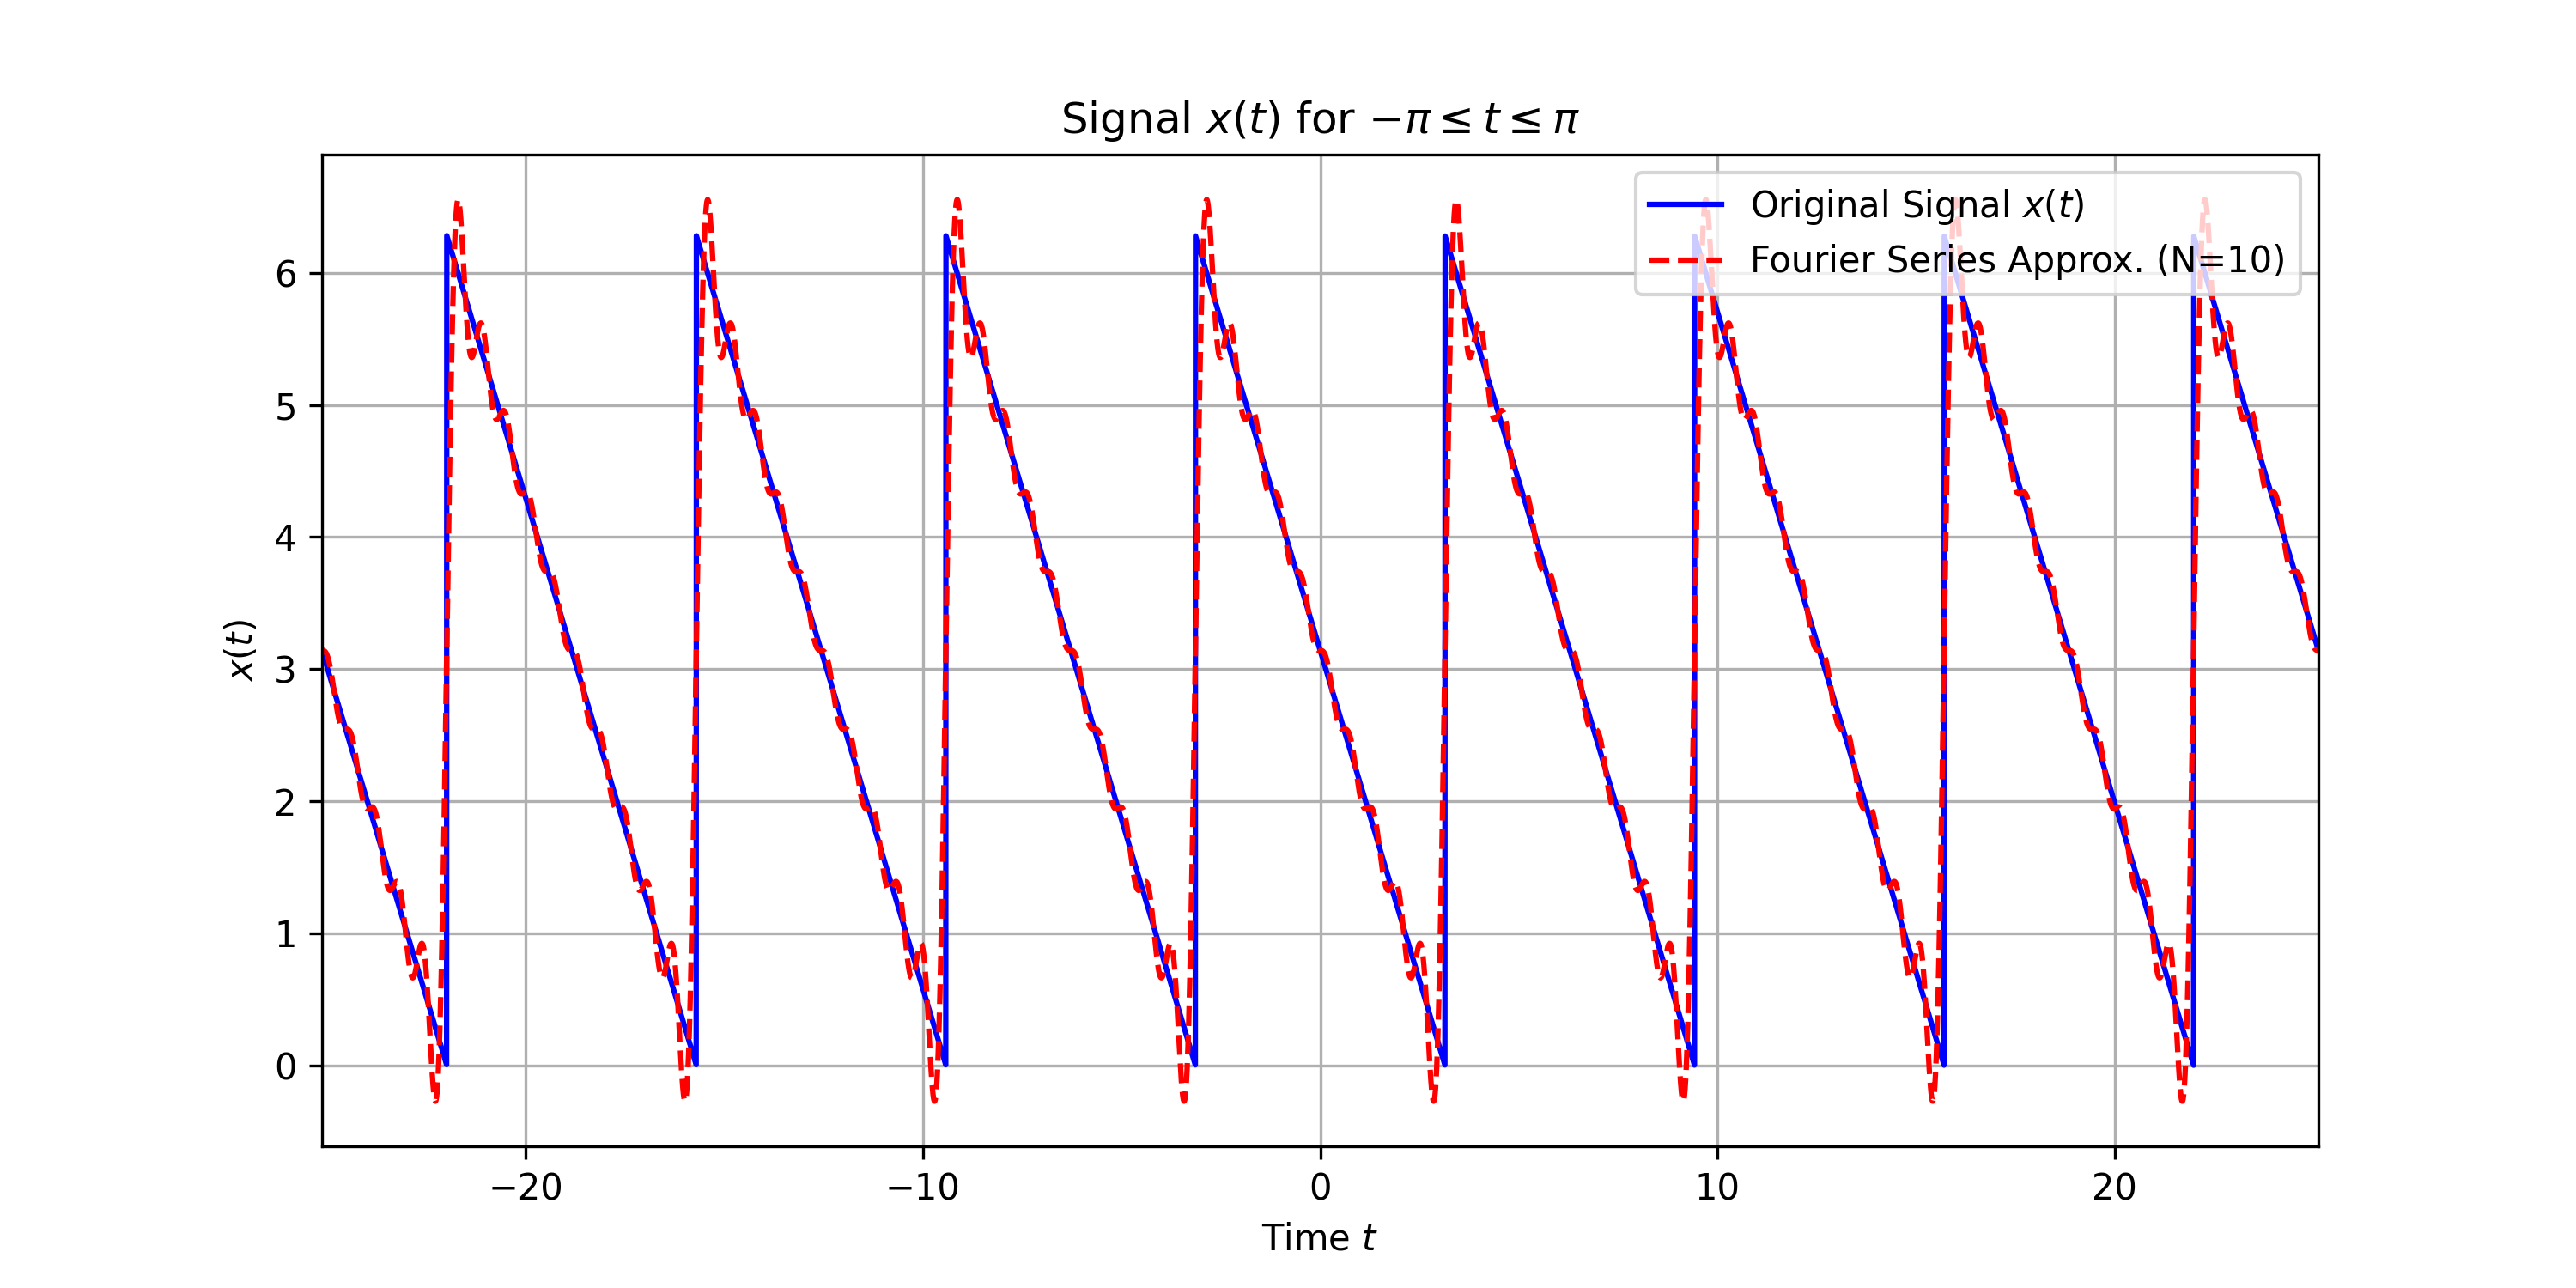
\includegraphics[width=0.9\textwidth]{images/problem_2_2.png}
\end{center}
\end{tosubmit}
% ==================== %

\newpage

% === Problem 2.3. === %
\begin{tosubmit}
\begin{subproblems}[start=3]
    \item \( x(t) = t^2 + \sin^3(\pi t);\; -1 \leq t \leq 1 \)
\end{subproblems}

\par\noindent\submitsolution
To find the Fourier series of the function \( x(t) = t^2 + \sin^3(\pi t) \) for \( -1 \leq t \leq 1 \), we first need to compute the Fourier coefficients.
The Fourier coefficients \( a_k \) are given by:
\[ a_k = \frac{1}{T} \int_{\langle T \rangle} x(t) e^{-j k \omega_0 t} \,dt \]

where \( T = 2 \) (the period of the function).

Calculating \( \omega_0 \):
\[ \omega_0 = \frac{2 \pi}{T} = \frac{2 \pi}{2} = \pi \]

Calculating \( a_0 \):
\begin{align*}
    a_0 &= \frac{1}{T} \int_{\langle T \rangle} x(t) e^{-j (0) \omega_0 t} \,dt \\
    &= \frac{1}{2} \int_{-1}^{1} (t^2 + \sin^3(\pi t)) \,dt \\
    &= \frac{1}{2} \int_{-1}^{1} t^2 \,dt + \frac{1}{2} \int_{-1}^{1} \sin^3(\pi t) \,dt \\
    &= \frac{1}{2} \sqbracket{ \frac{t^3}{3} }_{-1}^{1} + \frac{1}{2} (0) \quad \text{ since } \sin^3(\pi t) \text{ is odd function} \\
    &= \frac{1}{2} \sqbracket{ \frac{1^3}{3} - \frac{(-1)^3}{3} } + 0 \\
    &= \frac{1}{2} \cdot \frac{2}{3} \\
    a_0 &= \frac{1}{3}
\end{align*}

Calculating \( a_k \) for \( k \neq 0 \):
\begin{align*}
    a_k &= \frac{1}{T} \int_{\langle T \rangle} x(t) e^{-j k \omega_0 t} \,dt \\
    &= \frac{1}{2} \int_{-1}^{1} (t^2 + \sin^3(\pi t)) e^{-j k \pi t} \,dt \\
    a_k &= \frac{1}{2} \sqbracket{ \int_{-1}^{1} t^2 e^{-j k \pi t} \,dt + \int_{-1}^{1} \sin^3(\pi t) e^{-j k \pi t} \,dt }
\end{align*}

Define \[ I_1 = \int_{-1}^{1} t^2 e^{-j k \pi t} \,dt \quad \text{and} \quad I_2 = \int_{-1}^{1} \sin^3(\pi t) e^{-j k \pi t} \,dt \]
Hence, \[ a_k = \frac{1}{2} (I_1 + I_2) \].

\newpage

To solve the integral \( I_1 \), we can use integration by parts multiple times.
Using tabular integration by parts, we find:

\renewcommand{\arraystretch}{1.7}
\[
\begin{array}{c:c|c}
    \text{Sign} & \text{Derivative} & \text{Integral} \\
    \hline
    \hline
    + & t^2 & e^{-j \pi k t} \\
    - & 2t & \frac{1}{-j \pi k} e^{-j \pi k t} \\
    + & 2 & \frac{1}{(-j \pi k)^2} e^{-j \pi k t} \\
    - & 0 & \frac{1}{(-j \pi k)^3} e^{-j \pi k t} \\
    \hline
\end{array}
\]

Thus, we have:
\[ I_1 = \int t^2 e^{-j k \pi t} \,dt = \frac{t^2}{-j \pi k} e^{-j k \pi t} - \frac{2t}{(-j \pi k)^2} e^{-j k \pi t} + \frac{2}{(-j \pi k)^3} e^{-j k \pi t} \]

Evaluating this from \( -1 \) to \( 1 \) to find \( I_1 \):
\begin{align*}
    I_1 &= \sqbracket{ \textcolor[HTML]{1F77B4}{ \frac{t^2}{-j \pi k} e^{-j k \pi t} } - \textcolor[HTML]{FF7F0E}{ \frac{2t}{(-j \pi k)^2} e^{-j k \pi t} } + \textcolor[HTML]{2CA02C}{ \frac{2}{(-j \pi k)^3} e^{-j k \pi t} } }_{-1}^{1} \\
    &= \sqbracket{ \textcolor[HTML]{1F77B4}{ \frac{-2 \bcancel{j} \sin{\pi k}}{-\bcancel{j} \pi k} } - \textcolor[HTML]{FF7F0E}{ \frac{4 \cos{\pi k}}{(-j \pi k)^2} } + \textcolor[HTML]{2CA02C}{ \frac{-4 \bcancel{j} \sin{\pi k}}{(-\bcancel{j} \pi k)^3} } } \\
    &= \frac{-2 \sin{\pi k}}{-\pi k} - \frac{4 \cos{\pi k}}{(-j \pi k)^2} + \frac{-4 \sin{\pi k}}{j^2 (-\pi k)^3} \\
    I_1 &= \frac{2 \sin{\pi k}}{\pi k} + \frac{4 \cos{\pi k}}{(\pi k)^2} - \frac {4 \sin{\pi k}}{(\pi k)^3}
\end{align*}

Next, to solve the integral \( I_2 \), we can use the euler identity:
\[ \sin^3(x) = \set{ \frac{1}{2j} \paren{ e^{jx} - e^{-jx} } }^3 = -\frac{1}{8j} \paren{ e^{3jx} - 3e^{jx} + 3e^{-jx} - e^{-3jx} } \]

Thus, 
\begin{align*}
    I_2 &= \int_{-1}^{1} \sin^3(\pi t) e^{-j k \pi t} \,dt \\
    &= \int_{-1}^{1} -\frac{1}{8j} \paren{ e^{3j \pi t} - 3e^{j \pi t} + 3e^{-j \pi t} - e^{-3j \pi t} } e^{-j k \pi t} \,dt \\
    &= -\frac{1}{8j} \int_{-1}^{1} \paren{ e^{j \pi t (3 - k)} - 3e^{j \pi t (1 - k)} + 3e^{-j \pi t (1 + k)} - e^{-j \pi t (3 + k)} } \,dt \\
    &= -\frac{1}{8j} \sqbracket{ \frac{e^{j \pi t (3 - k)}}{j \pi (3 - k)} - \frac{3 e^{j \pi t (1 - k)}}{j \pi (1 - k)} + \frac{3 e^{-j \pi t (1 + k)}}{-j \pi (1 + k)} - \frac{e^{-j \pi t (3 + k)}}{-j \pi (3 + k)} }_{-1}^{1} \\
    &= -\frac{1}{ \cancel{8}^{\, 4} j } \sqbracket{ \frac{ \cancel{2} \bcancel{j} \sin{\pi (3 - k)}}{\bcancel{j} \pi (3 - k)} - \frac{3 \paren{ \cancel{2} \bcancel{j} \sin{\pi (1 - k)} }}{\bcancel{j} \pi (1 - k)} + \frac{3 \paren { -\cancel{2} \bcancel{j} \sin{\pi (1 + k)} }}{-\bcancel{j} \pi (1 + k)} - \frac{- \cancel{2} \bcancel{j} \sin{\pi (3 + k)}}{-\bcancel{j} \pi (3 + k)} } \\
    I_2 &= -\frac{1}{4j} \sqbracket{ \frac{\sin{\pi (3 - k)}}{\pi (3 - k)} - \frac{3 \sin{\pi (1 - k)}}{\pi (1 - k)} + \frac{3 \sin{\pi (1 + k)}}{\pi (1 + k)} - \frac{\sin{\pi (3 + k)}}{\pi (3 + k)} }
\end{align*}

\newpage

Therefore, we have:
\begin{align*}
    a_k &= \frac{1}{2} (I_1 + I_2) \\
    &= \frac{1}{ \cancel{2} } \sqbracket{ \frac{ \cancel{2} \sin{\pi k}}{\pi k} + \frac{ \cancel{4}^{\, 2} \cos{\pi k}}{(\pi k)^2} - \frac { \cancel{4}^{\, 2} \sin{\pi k}}{(\pi k)^3} } \\
    &\quad - \frac{1}{2} \cdot \frac{1}{4j} \sqbracket{ \frac{\sin{\pi (3 - k)}}{\pi (3 - k)} - \frac{3 \sin{\pi (1 - k)}}{\pi (1 - k)} + \frac{3 \sin{\pi (1 + k)}}{\pi (1 + k)} - \frac{\sin{\pi (3 + k)}}{\pi (3 + k)} } \\
    a_k &= \frac{\sin{\pi k}}{\pi k} + \frac{2 \cos{\pi k}}{(\pi k)^2} - \frac {2 \sin{\pi k}}{(\pi k)^3} \\
    &\quad - \frac{\sin{\pi (3 - k)}}{8j\pi (3 - k)} + \frac{3 \sin{\pi (1 - k)}}{8j\pi (1 - k)} - \frac{3 \sin{\pi (1 + k)}}{8j\pi (1 + k)} + \frac{\sin{\pi (3 + k)}}{8j\pi (3 + k)}
\end{align*}

Consider the value of \( a_k \), we can see that at \( \abs{ k } = 1 \) and \( \abs{ k } = 3 \), the terms will be undefined. Therefore, we need to calculate these four cases separately using limits.

\vspace{5mm}

For \( k = 1 \):
\begin{align*}
    a_1 &= \lim_{k \to 1} \sqbracket{ \frac{\sin{\pi k}}{\pi k} + \frac{2 \cos{\pi k}}{(\pi k)^2} - \frac {2 \sin{\pi k}}{(\pi k)^3} } \\
    &\quad + \lim_{k \to 1} \sqbracket{ -\frac{\sin{\pi (3 - k)}}{8j\pi (3 - k)} + \frac{3 \sin{\pi (1 - k)}}{8j\pi (1 - k)} - \frac{3 \sin{\pi (1 + k)}}{8j\pi (1 + k)} + \frac{\sin{\pi (3 + k)}}{8j\pi (3 + k)} } \\
    &= \paren{ 0 + \frac{2(-1)}{\pi^2} - 0 } + \paren{ -\frac{0}{16j\pi} + \lim_{k \to 1} \frac{3 \sin{\pi (1 - k)}}{8j\pi (1 - k)} - \frac{0}{16j\pi} + \frac{0}{32j\pi} } \\
    a_1 &= -\frac{2}{\pi^2} - \frac{3j}{8}
\end{align*}

For \( k = -1 \):
\begin{align*}
    a_{-1} &= \lim_{k \to -1} \sqbracket{ \frac{\sin{\pi k}}{\pi k} + \frac{2 \cos{\pi k}}{(\pi k)^2} - \frac {2 \sin{\pi k}}{(\pi k)^3} } \\
    &\quad + \lim_{k \to -1} \sqbracket{ -\frac{\sin{\pi (3 - k)}}{8j\pi (3 - k)} + \frac{3 \sin{\pi (1 - k)}}{8j\pi (1 - k)} - \frac{3 \sin{\pi (1 + k)}}{8j\pi (1 + k)} + \frac{\sin{\pi (3 + k)}}{8j\pi (3 + k)} } \\
    &= \paren{ 0 + \frac{2(-1)}{\pi^2} - 0 } + \paren{ -\frac{0}{16j\pi} + \frac{0}{6j\pi} - \lim_{k \to -1} \frac{3 \sin{\pi (1 + k)}}{8j\pi (1 + k)} + \frac{0}{32j\pi} } \\
    a_{-1} &= -\frac{2}{\pi^2} + \frac{3j}{8}
\end{align*}

Thus, we have:
\[ a_k = -\frac{2}{\pi^2} - \frac{3jk}{8} \text{ for } \abs{ k } = 1 \]

\vspace{5mm}

For \( k = 3 \):
\begin{align*}
    a_3 &= \lim_{k \to 3} \sqbracket{ \frac{\sin{\pi k}}{\pi k} + \frac{2 \cos{\pi k}}{(\pi k)^2} - \frac {2 \sin{\pi k}}{(\pi k)^3} } \\
    &\quad + \lim_{k \to 3} \sqbracket{ -\frac{\sin{\pi (3 - k)}}{8j\pi (3 - k)} + \frac{3 \sin{\pi (1 - k)}}{8j\pi (1 - k)} - \frac{3 \sin{\pi (1 + k)}}{8j\pi (1 + k)} + \frac{\sin{\pi (3 + k)}}{8j\pi (3 + k)} } \\
    &= \paren{ 0 + \frac{2(-1)}{(3\pi)^2} - 0 } + \paren{ -\lim_{k \to 3} \frac{\sin{\pi (3 - k)}}{8j\pi (3 - k)} + \frac{0}{-16j\pi} - \frac{0}{32j\pi} + \frac{0}{48j\pi} } \\
    a_3 &= -\frac{2}{9\pi^2} + \frac{j}{8}
\end{align*}

\newpage

For \( k = -3 \):
\begin{align*}
    a_{-3} &= \lim_{k \to -3} \sqbracket{ \frac{\sin{\pi k}}{\pi k} + \frac{2 \cos{\pi k}}{(\pi k)^2} - \frac {2 \sin{\pi k}}{(\pi k)^3} } \\
    &\quad + \lim_{k \to -3} \sqbracket{ -\frac{\sin{\pi (3 - k)}}{8j\pi (3 - k)} + \frac{3 \sin{\pi (1 - k)}}{8j\pi (1 - k)} - \frac{3 \sin{\pi (1 + k)}}{8j\pi (1 + k)} + \frac{\sin{\pi (3 + k)}}{8j\pi (3 + k)} } \\
    &= \paren{ 0 + \frac{2(-1)}{(3\pi)^2} - 0 } + \paren{ -\frac{0}{16j\pi} + \frac{0}{6j\pi} - \lim_{k \to -3} \frac{3 \sin{\pi (1 + k)}}{8j\pi (1 + k)} + \frac{0}{48j\pi} } \\
    a_{-3} &= -\frac{2}{9\pi^2} - \frac{j}{8}
\end{align*}

Thus, we have:
\[ a_k = -\frac{2}{9\pi^2} + \frac{jk}{24} \text{ for } \abs{ k } = 3 \]

\vspace{5mm}

For other values of \( k \) where \( \abs{ k } \neq 0, 1, 3 \):
\begin{align*}
    a_k &= \paren{ \frac{\sin{\pi k}}{\pi k} + \frac{2 \cos{\pi k}}{(\pi k)^2} - \frac {2 \sin{\pi k}}{(\pi k)^3} } \\
    &\quad + \paren{ - \frac{\sin{\pi (3 - k)}}{8j\pi (3 - k)} + \frac{3 \sin{\pi (1 - k)}}{8j\pi (1 - k)} - \frac{3 \sin{\pi (1 + k)}}{8j\pi (1 + k)} + \frac{\sin{\pi (3 + k)}}{8j\pi (3 + k)} } \\
    &= \paren{ 0 + \frac{2 (-1)^k}{(\pi k)^2} } + \paren{ - 0 + \frac{0}{8j\pi (3 - k)} + \frac{0}{8j\pi (1 - k)} - \frac{0}{8j\pi (1 + k)} + \frac{0}{8j\pi (3 + k)} } \\
    a_k &= \frac{2 (-1)^k}{k^2 \pi^2}
\end{align*}

Simplify \( a_k \):
\[
a_k = \begin{cases}
    \frac{1}{3} & k = 0 \\
    -\frac{2}{\pi^2} - \frac{3jk}{8} & \abs{ k } = 1 \\
    -\frac{2}{9\pi^2} + \frac{jk}{24} & \abs{ k } = 3 \\
    \frac{2 (-1)^k}{k^2 \pi^2} & \text{otherwise}
\end{cases}
\]

Therefore, the Fourier series expansion of \( x(t) \) is:
\[ \boxed{ x(t) = \paren{ \frac{1}{3} - \frac{40}{9\pi^2} } e^{j\pi t} + \sum_{\abs{ k } \neq 0, 1, 3} \frac{2 (-1)^k}{k^2 \pi^2} e^{j\pi t} } \]

By using Fourier series and Python approximation with \( N = 10 \) harmonics, we can approximate the signal as follows:
\begin{center}
    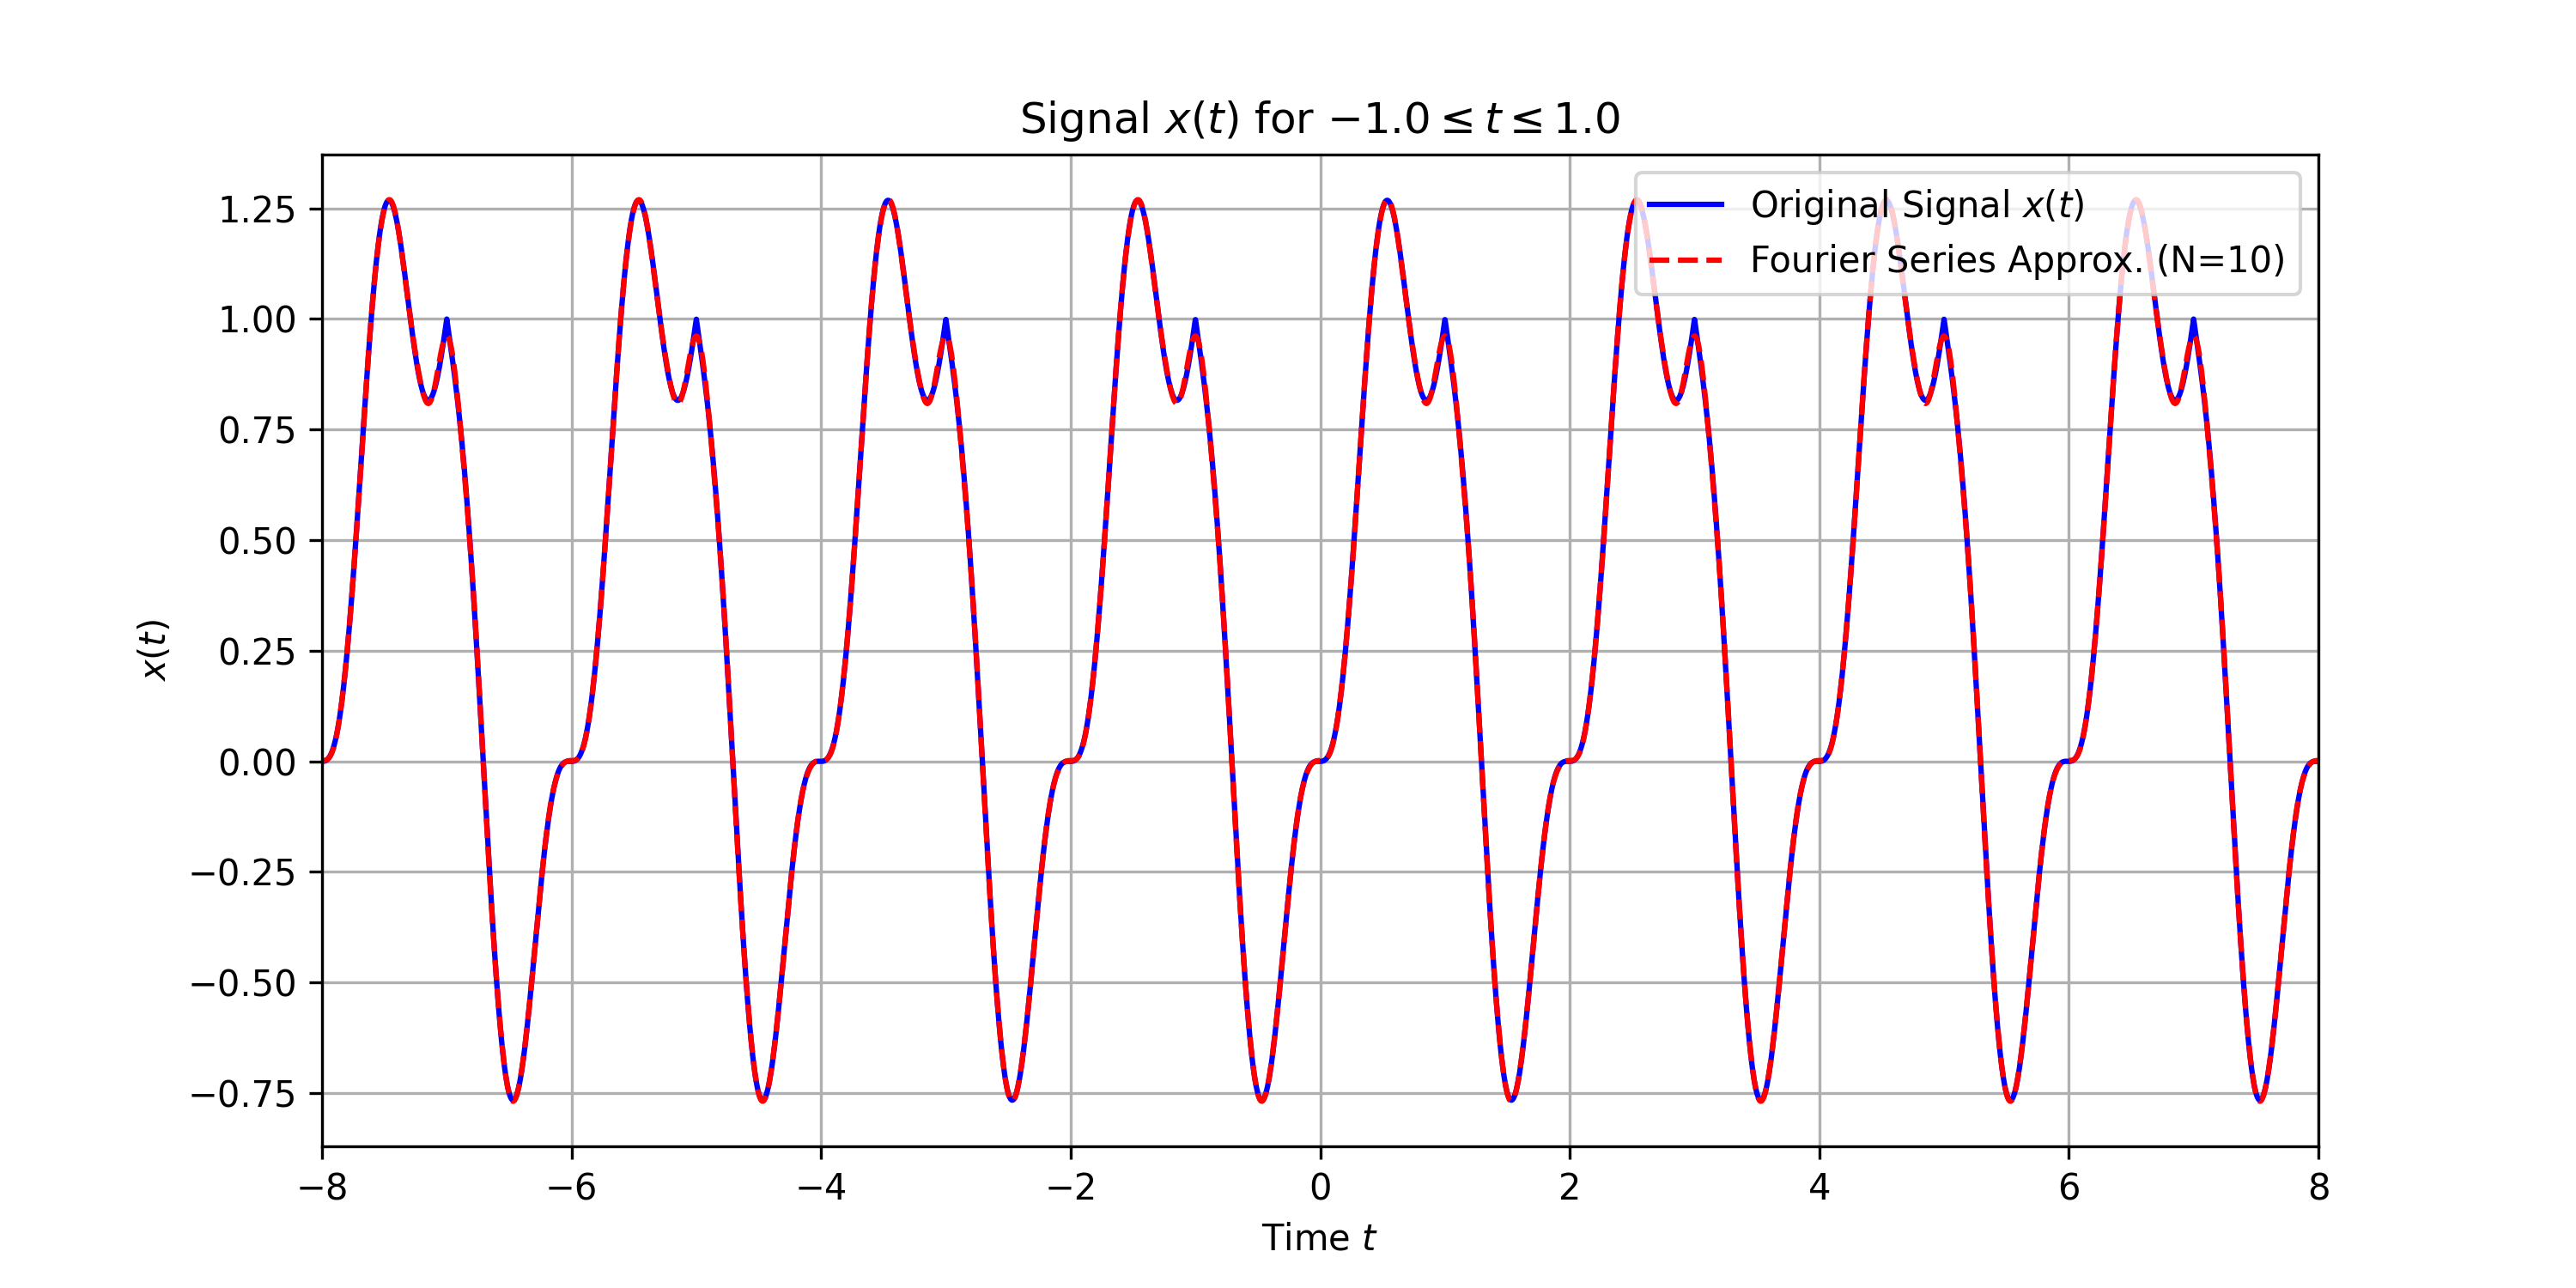
\includegraphics[width=0.9\textwidth]{images/problem_2_3.png}
\end{center}
\end{tosubmit}
% ==================== %
% ================================================================================ %


\end{document}